% !TeX program = xelatex
\documentclass[10pt,a4paper]{article}
\usepackage[a4paper,margin=18mm]{geometry}
\usepackage{iftex}
\ifPDFTeX
  \usepackage[T1]{fontenc}\usepackage[utf8]{inputenc}
  \IfFileExists{tgtermes.sty}{\usepackage{tgtermes}\usepackage{tgheros}}{\usepackage{times}\usepackage[scaled=0.92]{helvet}}
\else
  \usepackage{fontspec}\setmainfont{TeX Gyre Termes}\setsansfont{TeX Gyre Heros}
\fi
\usepackage{amsmath,amssymb,graphicx,array,booktabs,tabularx,caption,titlesec,fancyhdr,pifont,placeins}
\usepackage[table]{xcolor}
\usepackage[hidelinks]{hyperref}
\definecolor{ink2}{HTML}{52514E}\definecolor{rule}{HTML}{D9D8D3}\definecolor{head}{HTML}{1C5CAB}\definecolor{zebra}{HTML}{F5F7FB}
\definecolor{yes}{HTML}{0CA30C}\definecolor{no}{HTML}{B8B7B2}
\titleformat{\section}{\sffamily\large\bfseries\color{head}}{}{0pt}{}
\titleformat{\subsection}{\sffamily\normalsize\bfseries}{}{0pt}{}
\captionsetup{font={small,sf},labelfont={bf,color=head},labelsep=period,justification=justified,singlelinecheck=false}
\renewcommand{\thetable}{S\arabic{table}}\renewcommand{\thefigure}{S\arabic{figure}}
\setlength{\parindent}{0pt}\setlength{\parskip}{5pt}
\pagestyle{fancy}\fancyhf{}\renewcommand{\headrulewidth}{0pt}
\fancyfoot[C]{\sffamily\small\color{ink2}S\thepage}
\fancyhead[R]{\sffamily\scriptsize\color{ink2}Supplementary Information}
\newcommand{\Y}{\textcolor{yes}{\ding{51}}}\newcommand{\N}{\textcolor{no}{\ding{55}}}
\newcommand{\tabsetup}{\sffamily\footnotesize\rowcolors{2}{zebra}{white}\renewcommand{\arraystretch}{1.25}\arrayrulecolor{rule}}
\begin{document}
{\sffamily\small\color{head}\bfseries SUPPLEMENTARY FILE 1\par}\vspace{4pt}
{\sffamily\Large\bfseries Stage-Resolved Transcriptomic Analysis Reveals Distinct Molecular Programs Associated with Liver Fibrosis Severity\par}
\vspace{4pt}{\sffamily\small N.~Thanvitha\textsuperscript{1}, V.~Lakshmi Nikitha\textsuperscript{1}, K.~Venkata Dinesh\textsuperscript{1}, Biswajit Maity\textsuperscript{1}, Ashmita Dey\textsuperscript{1,*}\par}
{\sffamily\small \textsuperscript{1}Department of Computer Science and Engineering, SRM University-AP, Amaravati 522 240, Andhra Pradesh, India\par}
{\sffamily\small \textsuperscript{*}Correspondence: Ashmita Dey, \href{mailto:ashmita.de@srmap.edu.in}{\nolinkurl{ashmita.de@srmap.edu.in}}\par
}


\begin{figure}[h]\centering
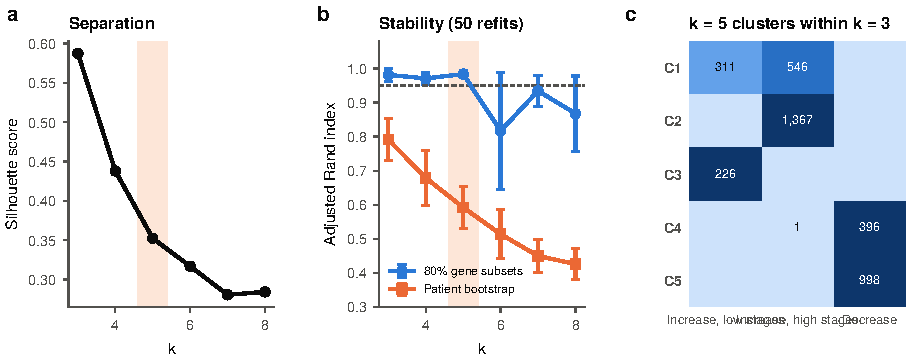
\includegraphics[width=\linewidth]{figs/figS1_k.pdf}
\caption{\textbf{Choice of cluster number and nesting of the five patterns.} (a) Silhouette score for $k=3$--8. (b) Mean adjusted Rand index ($\pm$ SD) over 50 refits on 80\% gene subsets and over 50 patient bootstraps; dashed line, 0.95 threshold; shaded, selected $k=5$. (c) Cross-tabulation of the $k=5$ clusters against the $k=3$ solution recomputed with identical settings (50 initialisations, seed 42); $k=3$ clusters are named from their centroid shapes. Re-running $k=5$ reproduced the published labels exactly (ARI 1.000); 91.9\% of genes fall in the $k=3$ cluster containing most of their $k=5$ cluster.}
\end{figure}


\begin{table}[h]\centering
\caption{\textbf{Dataset-specific preprocessing and final analysis eligibility.} Counts are patient-level observations within each study; the two analysis populations overlap and must not be added. Zero indicates no contribution to that analysis, not exclusion from the expression resource.}
\tabsetup
\begin{tabularx}{\linewidth}{l >{\raggedright\arraybackslash}p{0.21\linewidth} X cc}
\toprule
\rowcolor{white}\textbf{Dataset} & \textbf{Expression processing} & \textbf{Sample handling and eligibility} & \textbf{Fibrosis $n$} & \textbf{Disease $n$} \\
\midrule
GSE126848 & Raw counts; $\log_2$(CPM+1) & 12 obese-only samples excluded from the ordered analysis; no fibrosis stages. & 0 & 45 \\
GSE130970 & TPM; $\log_2$(TPM+1) & Five ambiguous classifications set to unclassified; remaining labels histology-derived. & 78 & 73 \\
GSE135251 & Counts; $\log_2$(CPM+1) & Broad NAFLD labels excluded, leaving no variation on the ordered axis. & 216 & 0 \\
GSE162694 & Raw counts; $\log_2$(CPM+1) & As GSE135251. & 143 & 0 \\
GSE167523 & Raw counts; $\log_2$(CPM+1) & All 98 NAFL/NASH observations eligible; no fibrosis stages. & 0 & 98 \\
GSE193066 & RLE-normalised counts; $\log_2$(count+1) & 164 biopsies resolved to 106 patients (28 same-stage pairs averaged; 30 first biopsy). & 106 & 0 \\
GSE240729 & Raw counts; $\log_2$(CPM+1) & All staged observations retained; no disease labels. & 67 & 0 \\
GSE269412 & Raw counts; $\log_2$(CPM+1) & Expression resource only; required annotations unavailable. & 0 & 0 \\
\midrule
\rowcolor{white}\textbf{Total} & & & \textbf{610} & \textbf{216} \\
\bottomrule
\end{tabularx}
\end{table}
\begin{table}[h]\centering
\caption{\textbf{Cluster-number diagnostics for all evaluated solutions.} Eligibility was assessed on unrounded means.}
\tabsetup
\begin{tabular}{ccccc}
\toprule
\rowcolor{white}$\boldsymbol{k}$ & \textbf{Silhouette} & \textbf{Gene-subset ARI (mean $\pm$ SD)} & \textbf{Patient-bootstrap ARI (mean $\pm$ SD)} & \textbf{Meets rule} \\
\midrule
3 & 0.5874 & 0.9811 $\pm$ 0.0183 & 0.7913 $\pm$ 0.0627 & Yes \\
4 & 0.4378 & 0.9708 $\pm$ 0.0174 & 0.6787 $\pm$ 0.0806 & Yes \\
\textbf{5} & \textbf{0.3522} & \textbf{0.9835 $\pm$ 0.0107} & \textbf{0.5919 $\pm$ 0.0623} & \textbf{Yes (selected)} \\
6 & 0.3167 & 0.8164 $\pm$ 0.1717 & 0.5137 $\pm$ 0.0727 & No \\
7 & 0.2804 & 0.9343 $\pm$ 0.0452 & 0.4495 $\pm$ 0.0478 & No \\
8 & 0.2841 & 0.8676 $\pm$ 0.1104 & 0.4257 $\pm$ 0.0455 & No \\
\bottomrule
\end{tabular}
\end{table}
\begin{table}[h]\centering
\caption{\textbf{Gene-prioritisation components and decision rules.} $S_g=P_g+T_g+X_g+F_g+B_g$ (maximum 9). Tier 1, $S_g\geq7$; Tier 2, $5\leq S_g<7$; Tier 3, $S_g<5$. Values rounded to three decimals; lower thresholds inclusive. The components share evidence and are not independent validations.}
\tabsetup
\begin{tabularx}{\linewidth}{c >{\raggedright\arraybackslash}p{0.22\linewidth} X}
\toprule
\rowcolor{white}\textbf{Score} & \textbf{Evidence} & \textbf{Assignment rule} \\
\midrule
$P_g$ & Association magnitude & 2: $|\mathrm{median}\,\rho|\geq0.40$; 1: $0.30\leq|\mathrm{median}\,\rho|<0.40$; 0 otherwise. \\
$T_g$ & F0--F4 endpoint separation & $\Delta_g=\bar z_{F4}-\bar z_{F0}$ must share the sign of the median correlation; then 2: $|\Delta_g|\geq1$; 1: $0.5\leq|\Delta_g|<1$; 0 otherwise. \\
$X_g$ & Largest adjacent-stage contrast & For the contrast with the largest $|\beta|$ (ties in stage order): A, $q<0.05$ and $|\beta|\geq0.2$; B, $\geq50\%$ of matched draws with $|\beta|\geq0.2$ and the same sign. 2 if A and B; 1 if one; 0 if neither. \\
$F_g$ & Fibrosis-only selection & 1 if selected on the fibrosis axis only; 0 otherwise. Not a claim of biological specificity. \\
$B_g$ & Functional annotation & Number of collections (GO BP, KEGG, Reactome, Hallmark) with a significant term containing the gene, via its direction group or full cluster. 2: $\geq2$; 1: one; 0: none. \\
\bottomrule
\end{tabularx}
\end{table}
\begin{table}[h]\centering
\caption{\textbf{Composition of the integrated knowledge graph and drug-annotation coverage.} Drug annotations were not inputs to the transcriptomic analyses.}
\tabsetup
\begin{tabular}{l r}
\toprule
\rowcolor{white}\textbf{Measure} & \textbf{Count} \\
\midrule
Total nodes / relationships & 126,480 / 35,152,951 \\
Broad entity categories / relationship types & 8 / 15 \\
KEGG (legacy) + Hallmark pathway nodes & 236 \\
Gene $\rightarrow$ KEGG/Hallmark pathway links (\texttt{IN\_PATHWAY}) & 20,031 \\
Pathway $\rightarrow$ NAFLD links (\texttt{IMPLICATED\_IN}) & 89 \\
Expression relationships & 32,471,042 \\
Fibrosis / disease-group progression links & 3,845 / 4,199 \\
Drug nodes (OptimusKG-derived) & 12,025 \\
\texttt{ACTS\_ON} relationships (OptimusKG-derived) & 20,674 \\
\texttt{TREATS} relationships (OptimusKG-derived) & 57,601 \\
Common source-list / action-list fields populated & 20,674 / 20,674 \\
Drug fields populated (of 12,025): SMILES / molecule type / max phase & 9,036 / 11,623 / 9,902 \\
Drug fields populated: approval / withdrawal flag / recovered name & 9,902 / 11,623 / 10,862 \\
OptimusKG drug--gene records with reference URLs / mechanism text (of 20,674) & 2,893 / 2,898 \\
Displayed annotation subgraph & 42 genes; 12 annotations; 154 links \\
\bottomrule
\end{tabular}
\par\vspace{2pt}{\footnotesize\sffamily\color{ink2}Drug nodes, molecular and clinical annotations, and drug--gene and drug--disease evidence were obtained through OptimusKG. A populated approval or withdrawal flag may be true or false; a phase field does not establish approval or efficacy for liver disease.}
\end{table}
\begin{figure}[p]\centering
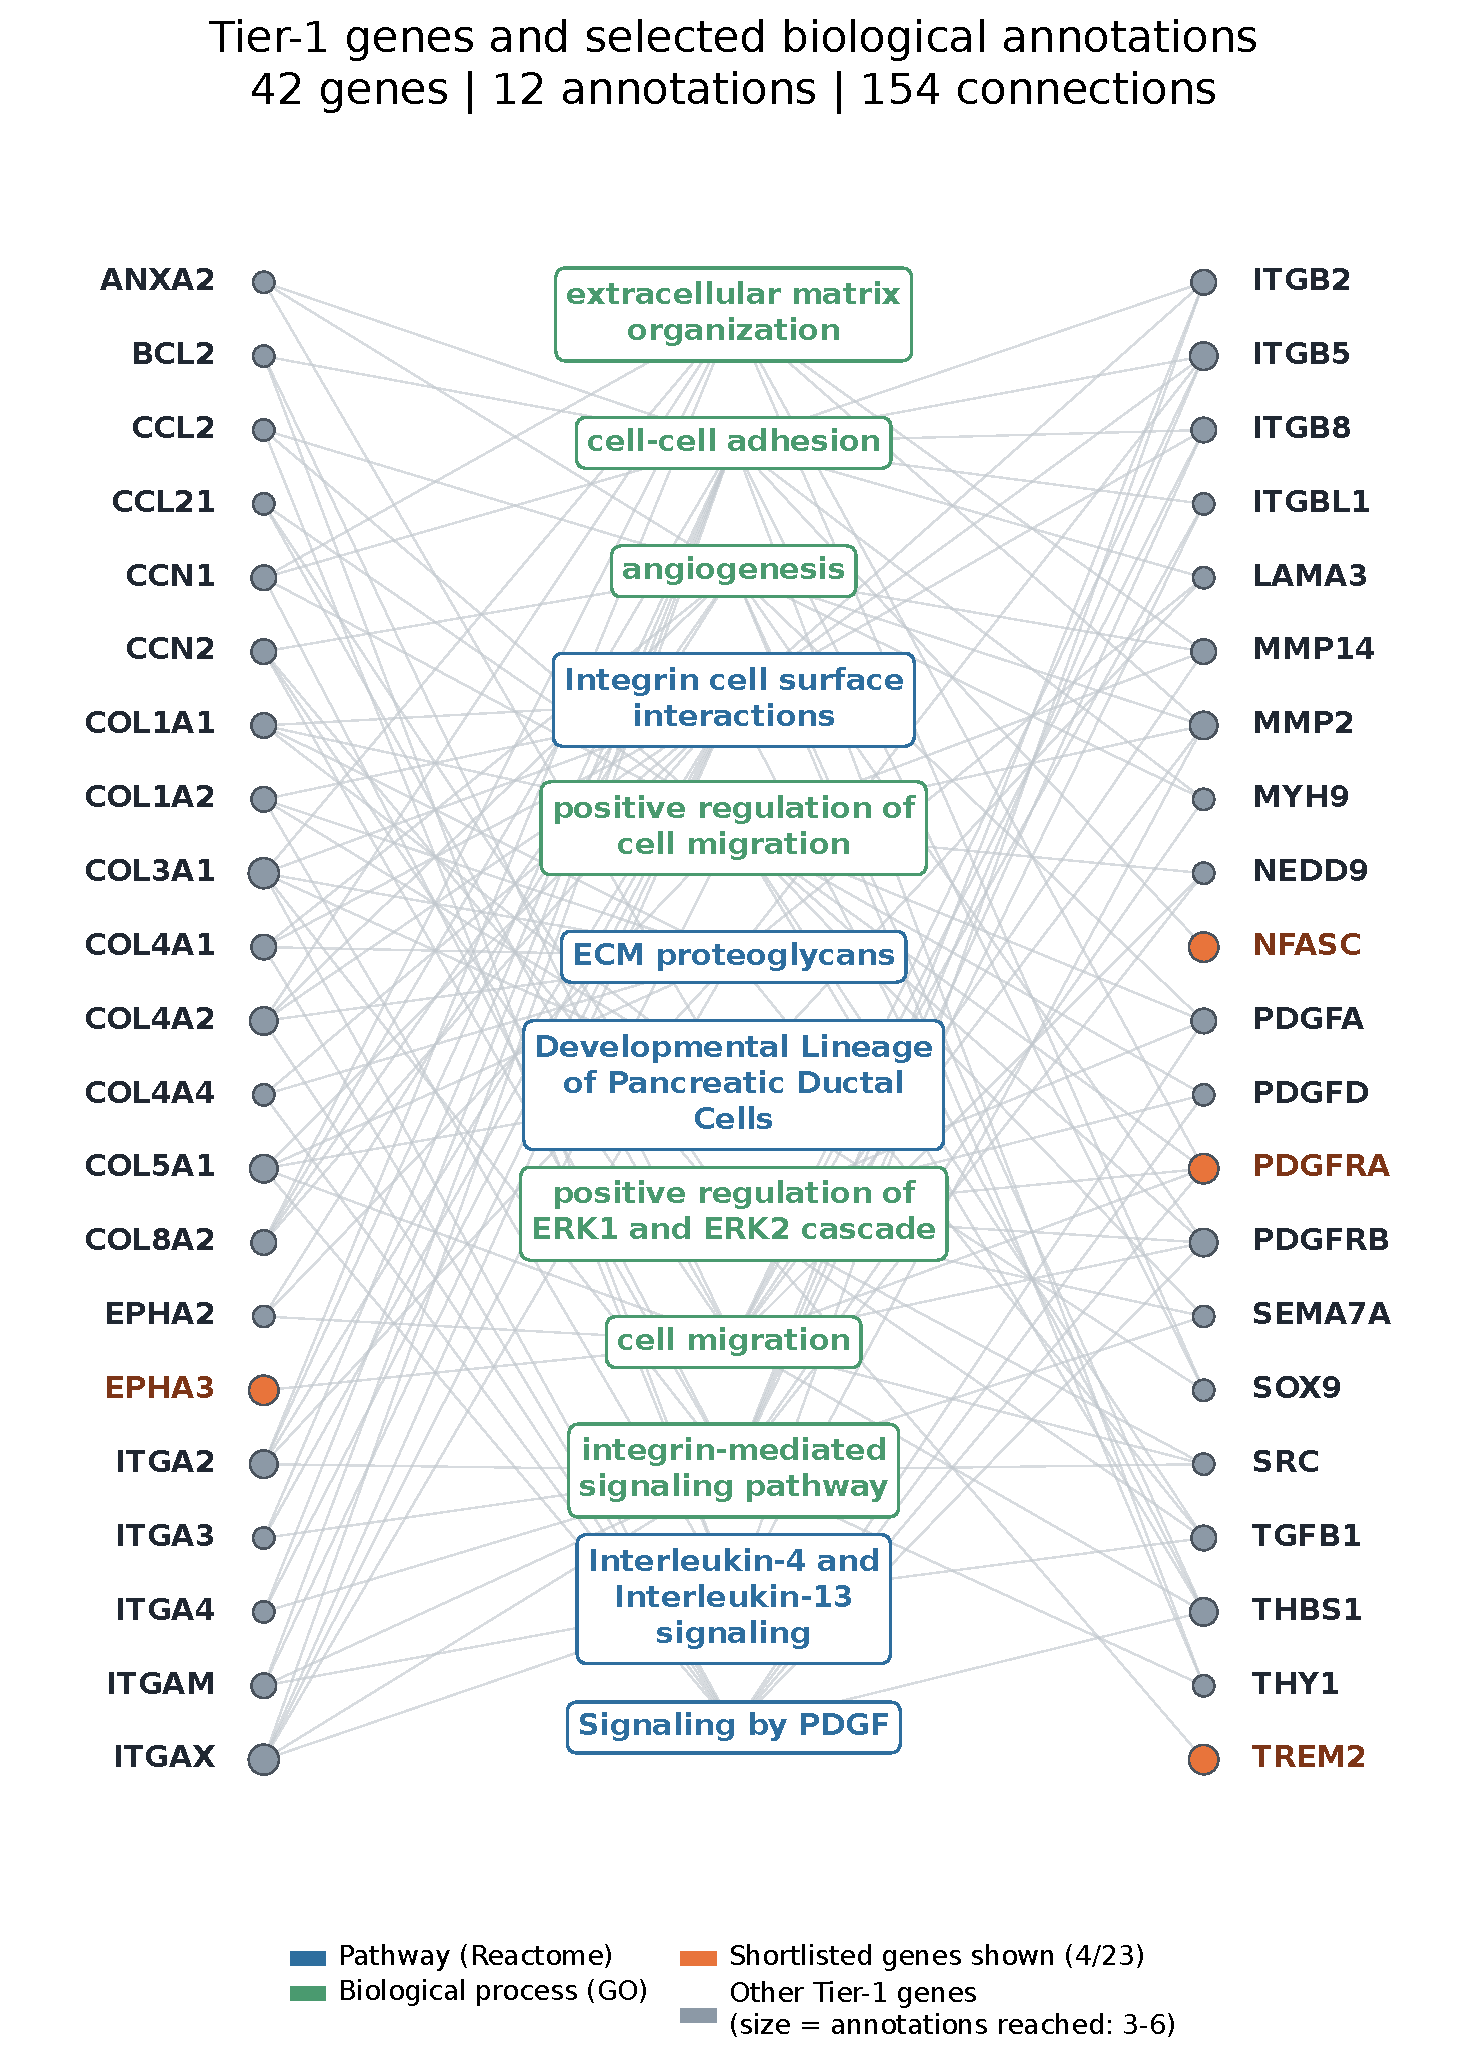
\includegraphics[width=\linewidth,height=0.82\textheight,keepaspectratio]{figs/figS3_kg_subgraph.pdf}
\caption{\textbf{Knowledge-graph annotation subgraph of Tier 1 genes.} Twelve non-redundant Pathway/BioProcess annotations over-represented among Tier 1 genes and the 42 Tier 1 genes linked to them through 154 curated relationships. Displayed genes reach at least three selected annotations or are shortlisted genes reaching at least one (\textit{PDGFRA}, \textit{EPHA3}, \textit{NFASC}, \textit{TREM2}). Links denote curated annotation membership, not physical or causal interactions.}
\end{figure}


\begin{table}[p]\centering
\caption{\textbf{Biological context of the 23 shortlisted genes.} Genes as in main-text Table~5, grouped by expression cluster. ``Established biological function'' summarises the general role of each gene product; ``previous evidence in liver disease'' gives referenced liver-disease associations, while entries marked ``General'' describe normal hepatic or cellular functions rather than evidence specific to liver disease; ``stage pattern'' describes the cluster's cross-sectional expression pattern across F0--F4 and does not imply a temporal sequence within patients. ---, no specific prior evidence in liver fibrosis was identified for this table; these genes are candidates for follow-up rather than established fibrosis genes.}
\label{tab:shortlistbio}
{\tabsetup
\begin{tabularx}{\linewidth}{@{}l c >{\raggedright\arraybackslash}X >{\raggedright\arraybackslash}X >{\raggedright\arraybackslash}p{3.6cm}@{}}
\toprule
\rowcolor{white}\textbf{Gene} & \textbf{Cluster} & \textbf{Established biological function} & \textbf{Previous evidence in liver disease} & \textbf{Stage pattern in this study} \\
\midrule
\textit{IL32} & C1 & Inflammatory cytokine signalling & Upregulated in NAFLD liver; candidate circulating biomarker$^{a}$ & Higher from F1, increasing with stage \\
\textit{EPHA3} & C1 & Ephrin receptor signalling & --- & Higher from F1, increasing with stage \\
\textit{LYZ} & C1 & Myeloid-associated immune function & --- & Higher from F1, increasing with stage \\
\textit{NFASC} & C1 & Cell adhesion and organisation & --- & Higher from F1, increasing with stage \\
\textit{PLPP4} & C1 & Lipid phosphate metabolism & --- & Higher from F1, increasing with stage \\
\textit{PDGFRA} & C2 & PDGF receptor signalling & PDGFR$\alpha^{+}$ scar-associated mesenchymal cells in human cirrhosis$^{b}$ & Increase, largest F3$\rightarrow$F4 \\
\textit{CACNA1C} & C2 & Calcium-channel signalling & --- & Increase, largest F3$\rightarrow$F4 \\
\textit{TPM4} & C2 & Cytoskeletal organisation & --- & Increase, largest F3$\rightarrow$F4 \\
\textit{PLK3} & C2 & Stress and cell-cycle regulation & --- & Increase, largest F3$\rightarrow$F4 \\
\textit{TAX1BP3} & C2 & Signalling scaffold & --- & Increase, largest F3$\rightarrow$F4 \\
\textit{TREM2} & C3 & Myeloid-cell-associated signalling & TREM2$^{+}$ scar-associated macrophages expand in human liver fibrosis$^{b}$ & Largest rise F0$\rightarrow$F1 \\
\textit{CDC45} & C3 & DNA replication & General: proliferation marker, not liver-specific & Largest rise F0$\rightarrow$F1 \\
\textit{HTR7} & C3 & Serotonin receptor signalling & --- & Largest rise F0$\rightarrow$F1 \\
\textit{FABP5} & C3 & Fatty-acid binding and lipid handling & --- & Largest rise F0$\rightarrow$F1 \\
\textit{TYMS} & C3 & Nucleotide biosynthesis & General: proliferation marker, not liver-specific & Largest rise F0$\rightarrow$F1 \\
\textit{OAT} & C4 & Amino-acid metabolism & --- & Decrease, largest F1$\rightarrow$F2 \\
\textit{KNG1} & C4 & Coagulation and inflammatory pathways & --- & Decrease, largest F1$\rightarrow$F2 \\
\textit{F2} & C4 & Coagulation & General: hepatic synthetic function & Decrease, largest F1$\rightarrow$F2 \\
\textit{SULT1E1} & C5 & Steroid metabolism & General: hepatic metabolic function & Decrease, largest F3$\rightarrow$F4 \\
\textit{SLC38A4} & C5 & Amino-acid transport & General: hepatic transport function & Decrease, largest F3$\rightarrow$F4 \\
\textit{CYP2C19} & C5 & Xenobiotic metabolism & Activity decreases with NAFLD severity$^{c}$ & Decrease, largest F3$\rightarrow$F4 \\
\textit{ACADSB} & C5 & Branched-chain amino-acid and fatty-acid metabolism & --- & Decrease, largest F3$\rightarrow$F4 \\
\textit{MME} & C5 & Membrane metalloprotease & --- & Decrease, largest F3$\rightarrow$F4 \\
\bottomrule
\end{tabularx}}
\par\smallskip{\sffamily\scriptsize $^{a}$Baselli GA, et al. Liver transcriptomics highlights interleukin-32 as novel NAFLD-related cytokine and candidate biomarker. Gut. 2020;69(10):1855--66. $^{b}$Ramachandran P, et al. Resolving the fibrotic niche of human liver cirrhosis at single-cell level. Nature. 2019;575(7783):512--8. $^{c}$Fisher CD, et al. Hepatic cytochrome P450 enzyme alterations in humans with progressive stages of nonalcoholic fatty liver disease. Drug Metab Dispos. 2009;37(10):2087--94.\par}
\end{table}

% \clearpage
% \section*{Supplementary Methods}
% Implementation details supplementing the main-text Methods.

% \subsection*{Implementation details}
% \textbf{Processing order.} Duplicate raw identifiers were resolved (first occurrence retained); identifiers were mapped to Ensembl and unmappable or PAR-Y records excluded; distinct identifiers mapping to the same sample--gene pair were summed; the study-appropriate transformation was applied (CPM library totals computed before mapping and filtering); each gene was standardised within study; and patient-level biopsy selection or averaging followed. Equal-stage repeat biopsies were averaged on the standardised scale without restandardisation.

% \textbf{Implementation checks for scoring.} For $X_g$, a missing full-data $q$-value did not satisfy the substantial-difference condition, and missing matched evidence halted scoring rather than defaulting to zero. In the final analysis all 3,845 fibrosis-associated genes had finite coefficients and $q$-values for all four contrasts and matched evidence for the selected contrast. Independently reconstructed P/T/X/F/B scores agreed with the analysis table for all 3,845 genes.

% \textbf{Graph verification.} All 8,044 progression relationships and their association properties were compared with the analysis exports, and the 154 displayed gene--annotation connections were checked by endpoint identifiers and relationship type.

% \textbf{Reference-file provenance.} Gene mapping used \texttt{hgnc\_complete\_set.txt} (file dated 20 August 2026; most recent record modification 18 August 2026); the knowledge layer used the OptimusKG parquet files (dated 1 September 2026; source deposit doi:10.7910/DVN/IYNGEV); functional annotation used MSigDB 2024.1.Hs. Formal release identifiers and expression-data download dates were not recorded; SHA-256 checksums of the retained HGNC, OptimusKG and MSigDB files are provided in \texttt{source\_checksums.txt} and in the code repository (\texttt{docs/provenance/SOURCE\_CHECKSUMS.txt}).



% \clearpage
% \subsection*{Reference-file SHA-256 checksums}
% The accompanying \texttt{source\_checksums.txt} contains the reference-file manifest recorded on 21 October 2026 after the analysis. The entries below reproduce that record for the HGNC dictionary and 14 OptimusKG parquet files; on 4 November 2026 all 15 checksums were re-checked and still matched the retained files, and checksums of the four MSigDB 2024.1 gene-set files used for enrichment (files dated 3 October 2026) were added. The same manifest is in the code repository as \texttt{docs/provenance/SOURCE\_CHECKSUMS.txt}. Paths are relative to the analysis input directory; filesystem modification dates and hashes identify retained files, not official release dates. CTD inputs supported the pathway--NAFLD graph annotations and are not listed in this reference-file manifest.

% \begingroup\footnotesize
% \noindent\nolinkurl{data/raw/hgnc_complete_set.txt}\par
% \noindent\texttt{4ad72ffc6bca0d0858bb7234cfb3c7b1fb10e8e693e2f8d5c0842b4cfb03e748}\par
% \smallskip
% \noindent\nolinkurl{data/optimuskg/biological_process.parquet}\par
% \noindent\texttt{02e41948a5ae33cc960a0030affdb60d360ceb38c9abfb05c614d9e62566bfd4}\par
% \smallskip
% \noindent\nolinkurl{data/optimuskg/biological_process_gene.parquet}\par
% \noindent\texttt{1f84ee31ce9fbdd02375650caa926d5ca424b6d5e5afb65cad688ed5f944e00f}\par
% \smallskip
% \noindent\nolinkurl{data/optimuskg/disease.parquet}\par
% \noindent\texttt{46b41e6553e7f0cdb2a787a6ecbf0062f6f1e51173b91331b2a77978d4a104a8}\par
% \smallskip
% \noindent\nolinkurl{data/optimuskg/disease_disease.parquet}\par
% \noindent\texttt{31f6666f975bcd78f0b9824de7f8e5059b3d82bdfe65abe271ac6f446779de24}\par
% \smallskip
% \noindent\nolinkurl{data/optimuskg/disease_gene.parquet}\par
% \noindent\texttt{3fb5df3f41ee917438826c2e98a21cc20dce172746fed32000ef477d88a33ac3}\par
% \smallskip
% \noindent\nolinkurl{data/optimuskg/disease_phenotype.parquet}\par
% \noindent\texttt{82e5c360adec86b95942c37d661771a5009f31df63061eea10e26c115643f637}\par
% \smallskip
% \noindent\nolinkurl{data/optimuskg/drug.parquet}\par
% \noindent\texttt{6b735706a094753f295f0925ac7403338a28ae6bf7b58d7a586f1644f88be51c}\par
% \smallskip
% \noindent\nolinkurl{data/optimuskg/drug_disease.parquet}\par
% \noindent\texttt{8fa670c3292eb45c202d1abf31667135708ef994c71f0a32e0d46320b24b802d}\par
% \smallskip
% \noindent\nolinkurl{data/optimuskg/drug_gene.parquet}\par
% \noindent\texttt{ab0b95d4805f3f085b703cce554b2064641b620bd8d13297fdaea2bf82b7cb4b}\par
% \smallskip
% \noindent\nolinkurl{data/optimuskg/gene.parquet}\par
% \noindent\texttt{4d394d15b6fdcaf25b110a7d4db78b7cb17c8de80efbde3255fbbe07087a0cd1}\par
% \smallskip
% \noindent\nolinkurl{data/optimuskg/gene_gene.parquet}\par
% \noindent\texttt{a1b12cfba84904ec8403f4069aa2f5c947ce204c23aa7c6e7c41b8a79c68207a}\par
% \smallskip
% \noindent\nolinkurl{data/optimuskg/pathway.parquet}\par
% \noindent\texttt{c27f5947c74965d0406bf818554d9d51ec859615594365f30e253e297f771682}\par
% \smallskip
% \noindent\nolinkurl{data/optimuskg/pathway_gene.parquet}\par
% \noindent\texttt{80e8d10cd87fb10be6fc392221c4910e4b116a70a14f410dd75a4524da298493}\par
% \smallskip
% \noindent\nolinkurl{data/optimuskg/phenotype.parquet}\par
% \noindent\texttt{a0dc2ed859e0f6965257029ea600b5f5069f9e92444179e939c0a57360a8674a}\par
% \smallskip
% \noindent\nolinkurl{data/genesets/c2.cp.kegg_legacy.v2024.1.Hs.symbols.gmt}\par
% \noindent\texttt{06a5d7f82d90a0a6a2e464579d049fc42d279fc23fa9f79a956e56c4a442447f}\par
% \smallskip
% \noindent\nolinkurl{data/genesets/c2.cp.reactome.v2024.1.Hs.symbols.gmt}\par
% \noindent\texttt{9ea1b5e656597daf423e41c5ebcaa9892bfedf3292fff768605d7b0d5e5e9703}\par
% \smallskip
% \noindent\nolinkurl{data/genesets/c5.go.bp.v2024.1.Hs.symbols.gmt}\par
% \noindent\texttt{71df041c352cc810c11847db328bb94925c5448a009f310d224f2e8baa60b792}\par
% \smallskip
% \noindent\nolinkurl{data/genesets/h.all.v2024.1.Hs.symbols.gmt}\par
% \noindent\texttt{ee2463540042078bfa3f67828e1e223bb354446d9fbb4d22845866835ba5c772}\par
% \smallskip
% \endgroup


\clearpage
\section*{Additional-cohort replication}
The discovery gene set and prioritisation were frozen before evaluation in the three cohorts below; these datasets did not enter discovery gene selection, clustering, scoring or graph construction. Cohorts were selected through targeted screening before examining validation results, based on eligibility, usable clinical annotations and gene coverage. All reported gene-level tests use one broad-universe BH correction per cohort.

\begin{table}[htbp]\centering\tabsetup
\caption{\textbf{Eligibility and testing families for the three additional cohorts.} Stage counts refer to eligible patients, not all deposited samples.}
\begin{tabularx}{\linewidth}{@{}lXXX@{}}
\toprule
Feature & GSE225740 & GSE213621 & GSE268273 \\
\midrule
Source observations & 93 & 368 & 109 \\
Eligible patients & 87 & 299 & 109 \\
Exclusions & 6 missing fibrosis stage & 69 controls & None \\
Stage distribution & F0:27; F1:26; F2:15; F3:13; F4:6 & F0--F1:97; F2:107; F3--F4:95 & F0:36; F1:41; F2:13; F3:14; F4:5 \\
Source scale & Raw counts & FPKM & Deposited normalised log expression \\
Transformation & $\log_2(\mathrm{CPM}+1)$ & $\log_2(\mathrm{FPKM}+1)$ & Retained on deposited scale \\
Testable BH family & 13,790 & 13,358 & 11,871 \\
Shortlisted genes unavailable & None & EPHA3, SULT1E1, KNG1, CYP2C19 & CDC45, TREM2, HTR7, CACNA1C, PLPP4 \\
Clinical context & Indiana NAFLD biopsy cohort & Duke NAFLD biopsy cohort & 69 IMID-NAFLD and 40 classic-NAFLD cases \\
\bottomrule
\end{tabularx}
\end{table}

\FloatBarrier
\begin{table}[htbp]\centering\tabsetup
\caption{\textbf{Stage associations of the frozen 23 shortlisted genes.} Cells show Spearman $\rho$ (BH-adjusted $q$). Bold cells indicate concordant $q<0.05$ based on unrounded values; --- indicates untestable. BH families are those in Table~S6. Grouped stages in GSE213621 remain grouped.}
\begin{tabularx}{\linewidth}{@{}l*{3}{>{\centering\arraybackslash}X}@{}}
\toprule
Gene & GSE225740 & GSE213621 & GSE268273 \\
\midrule
\textit{IL32} & $\boldsymbol{0.498\;(7.20\times10^{-5})}$ & $\boldsymbol{0.212\;(0.002)}$ & $\boldsymbol{0.470\;(1.44\times10^{-5})}$ \\
\textit{EPHA3} & $\boldsymbol{0.586\;(1.85\times10^{-6})}$ & --- & $\boldsymbol{0.586\;(1.03\times10^{-8})}$ \\
\textit{LYZ} & $\boldsymbol{0.315\;(0.015)}$ & $0.034\;(0.688)$ & $0.215\;(0.079)$ \\
\textit{NFASC} & $\boldsymbol{0.464\;(2.25\times10^{-4})}$ & $\boldsymbol{0.494\;(5.03\times10^{-17})}$ & $\boldsymbol{0.516\;(1.23\times10^{-6})}$ \\
\textit{PLPP4} & $\boldsymbol{0.356\;(0.006)}$ & $\boldsymbol{0.325\;(3.11\times10^{-7})}$ & --- \\
\textit{PDGFRA} & $\boldsymbol{0.481\;(1.28\times10^{-4})}$ & $\boldsymbol{0.337\;(8.86\times10^{-8})}$ & $\boldsymbol{0.382\;(6.83\times10^{-4})}$ \\
\textit{CACNA1C} & $\boldsymbol{0.456\;(2.98\times10^{-4})}$ & $\boldsymbol{0.443\;(1.91\times10^{-13})}$ & --- \\
\textit{TPM4} & $\boldsymbol{0.422\;(9.14\times10^{-4})}$ & $0.097\;(0.195)$ & $\boldsymbol{0.389\;(5.12\times10^{-4})}$ \\
\textit{PLK3} & $\boldsymbol{0.332\;(0.010)}$ & $\boldsymbol{0.210\;(0.002)}$ & $\boldsymbol{0.384\;(6.35\times10^{-4})}$ \\
\textit{TAX1BP3} & $\boldsymbol{0.499\;(7.01\times10^{-5})}$ & $\boldsymbol{0.190\;(0.005)}$ & $\boldsymbol{0.490\;(5.07\times10^{-6})}$ \\
\textit{TREM2} & $\boldsymbol{0.416\;(0.001)}$ & $0.101\;(0.171)$ & --- \\
\textit{CDC45} & $\boldsymbol{0.281\;(0.030)}$ & $\boldsymbol{0.189\;(0.006)}$ & --- \\
\textit{HTR7} & $\boldsymbol{0.355\;(0.006)}$ & $\boldsymbol{0.238\;(3.33\times10^{-4})}$ & --- \\
\textit{FABP5} & $\boldsymbol{0.412\;(0.001)}$ & $0.001\;(0.994)$ & $\boldsymbol{0.593\;(5.76\times10^{-9})}$ \\
\textit{TYMS} & $\boldsymbol{0.472\;(1.76\times10^{-4})}$ & $\boldsymbol{0.390\;(2.89\times10^{-10})}$ & $\boldsymbol{0.462\;(2.19\times10^{-5})}$ \\
\textit{OAT} & $-0.232\;(0.077)$ & $\boldsymbol{-0.346\;(3.86\times10^{-8})}$ & $\boldsymbol{-0.544\;(2.37\times10^{-7})}$ \\
\textit{KNG1} & $-0.031\;(0.839)$ & --- & $-0.081\;(0.565)$ \\
\textit{F2} & $\boldsymbol{-0.292\;(0.024)}$ & $\boldsymbol{-0.239\;(3.03\times10^{-4})}$ & $\boldsymbol{-0.349\;(0.002)}$ \\
\textit{SULT1E1} & $-0.212\;(0.108)$ & --- & $\boldsymbol{-0.285\;(0.016)}$ \\
\textit{SLC38A4} & $-0.247\;(0.058)$ & $\boldsymbol{-0.162\;(0.020)}$ & $\boldsymbol{-0.336\;(0.003)}$ \\
\textit{CYP2C19} & $\boldsymbol{-0.483\;(1.18\times10^{-4})}$ & --- & $\boldsymbol{-0.411\;(2.19\times10^{-4})}$ \\
\textit{ACADSB} & $\boldsymbol{-0.377\;(0.003)}$ & $\boldsymbol{-0.251\;(1.42\times10^{-4})}$ & $\boldsymbol{-0.459\;(2.64\times10^{-5})}$ \\
\textit{MME} & $\boldsymbol{-0.440\;(5.22\times10^{-4})}$ & $\boldsymbol{-0.320\;(4.81\times10^{-7})}$ & $\boldsymbol{-0.341\;(0.003)}$ \\
\bottomrule
\end{tabularx}
\end{table}
\FloatBarrier

\subsection*{Replication inputs, implementation and boundaries}
GSE225740 contributed 87 of 93 clinical biopsies; six lacked fibrosis stage. Its supplied phenotype table and GEO annotations were matched by patient identifier. GSE213621 supplied 299 NAFLD cases and 69 controls; only cases entered the stage test. Its F0--F1, F2 and F3--F4 labels were treated as three ordered categories. GSE268273 supplied 109 biopsy-labelled cases, comprising 69 patients with immune-mediated inflammatory conditions and 40 classic-NAFLD cases. These are disease comparators, not healthy controls. Recruitment sources were described by Powell et al. (doi:10.1038/s41467-023-37209-1), Chen et al. (doi:10.1016/j.jcmgh.2022.12.008), and Garc\'ia-Nieto et al. (doi:10.1016/j.jhepr.2024.101167), respectively.

Expression columns were matched bijectively to metadata, with no identical complete expression profiles or nonfinite expression entries detected. The first raw-identifier duplicate was retained; GSE213621 contained five duplicate raw rows. Version suffixes and PAR-Y rows were removed before mapped-gene aggregation. Count-library totals preceded mapping. Already-log GSE268273 values were not transformed to CPM. In the absence of raw-read reprocessing, source alignment and read-level quality were not independently verified. In particular, the GSE213621 processing narrative contains inconsistent assembly statements, so these were not treated as verified human alignment specifications.

The harmonised eligible universe was intersected with each cohort's measured, nonconstant genes. Each cohort used two-sided Spearman tests, average ranks for ties, the asymptotic $t$ approximation on $n-2$ degrees of freedom, and one BH correction across all its testable eligible genes. No gene selection, ranking or coefficient fitting was performed using the validation outcomes. Directional agreement compares the validation correlation sign with the frozen discovery median correlation; replication additionally requires $q<0.05$. Missing and constant measurements receive no test and do not count as opposite associations. Tests were unadjusted for clinical covariates and do not establish specificity to fibrosis or independence from cell composition.

No shared GSM was detected between eligible validation samples and the eight discovery cohorts or between the three selected validation cohorts. Available BioSample and SRA experiment identifiers also showed no overlap; GSE225740 lacks these identifiers, so those comparisons were unassessable. Primary-study recruitment descriptions support distinct cohorts, but de-identification prevents proof of donor-level nonoverlap. The original GSE225740 paper's separate literature meta-analysis and the additional public datasets analysed in the GSE213621 source article were not imported as new validation patients.

Validation used an official HGNC complete-set snapshot archived on retrieval, 7 November 2026, separately from the discovery reference. The exact snapshot used for the initial validation mapping could not be retrospectively identified; repeating the analysis with the archived snapshot reproduced all selected-gene testability sets, correlations, $p$-values and broad-universe $q$-values to numerical precision. Its retrieval date is not an official release date. SHA-256:
\begin{quote}\footnotesize\texttt{3944cdad7affce5bc2c7d63d7079d7e68762ed28ef414fc287cc0f57c4b0d78f}\end{quote}
Source URLs, filenames and hashes are retained in \nolinkurl{validation_source_manifest.csv}; gene-level results for all 3,845 original fibrosis-associated genes, including missing and nonsignificant observations, are supplied in \nolinkurl{validation_gene_results.csv}. This file reports only the three selected cohorts and the agreed broad-universe correction. Computational checks used Python 3.12.3, NumPy 2.5.3, pandas 3.0.5 and SciPy 1.18.1; openpyxl 3.1.5 read the deposited spreadsheet. Scalar Spearman calculations and independent BH calculations reproduced the reported gene-level statistics.

\end{document}
